\documentclass[11pt]{article}
\usepackage[margin=1in]{geometry}
\usepackage{amsmath,amssymb}
\usepackage{booktabs,graphicx,caption}
\usepackage[hidelinks]{hyperref}
\setlength{\parskip}{4pt}

\title{Embodied Technical Progress in AI versus Regular Capital:\\
Dynamics under Log Utility, Habits, and Rule-of-Thumb Consumers}
\author{Research note (draft)}
\date{October 2026}

\begin{document}
\maketitle

\begin{abstract}
\noindent Embodied progress lowers the price of new capital in efficiency units, so it raises output only as
capital is installed. This note compares the dynamics of the real interest rate, GDP, consumption, the investment
share of GDP, the real wage and the labor share after embodied progress in AI capital and in regular capital, under four
flex-price household blocks, all with log utility: a representative household; the same with habits; habits
plus 50 percent \emph{hand-to-mouth} households, who consume their labor income; and habits plus 50 percent
\emph{constant savers}, who save a constant share of gross income. Every shock is a one-time level shift that raises long-run
GDP by 10 percent. GDP is gross value added, and adjustment costs are counted as investment. Adjustment costs are half the earlier
baseline, and depreciation is equal for both capital stocks. Output builds slowly even so. After a surprise jump, GDP at year 10 is 45--55 percent of its long-run gain
(regular capital 53--55, AI 45--49), and after an S-curve complete at year 5 it is 34--41 percent.
The investment share of GDP rises by 0.8--1.4 points, and for AI it stays about 1.2--1.4 points higher for more than 20 years. For regular capital the rise is transitory. Habits
shape the real-rate response more than the rule-of-thumb types do. The two rule-of-thumb types give nearly the same results as each other and as habits alone.
\end{abstract}

\section{Setup}

\paragraph{Technology and shocks.} Production is a Cobb-Douglas bundle of regular capital and labor inside a CES
aggregate with AI capital ($\varepsilon=1.5$, so AI substitutes for the bundle). Capital accumulates in efficiency units, and
a new unit costs $P_j$. \emph{Embodied} progress lowers $P_j$: regular capital's price falls 22 percent (a 29 percent improvement in $1/P_K$) and AI's 71 percent
(a 3.4-fold improvement), so that each shock raises long-run output by 10 percent. Depreciation is equal for both stocks, $d_A=d_K=6.6$ percent.
Trend growth is 1.5 percent, hours are fixed and the initial real rate is 7.5 percent. Three timings:
\begin{itemize}
\item a surprise \emph{jump} at $t=0$;
\item an \emph{S-curve}, announced at $t=0$, that rises as $\tfrac12[1-\cos(\pi t/5)]$ and is complete by year 5;
\item \emph{half/half}: half the improvement as a jump, half along the 5-year S-curve.
\end{itemize}

\paragraph{Adjustment costs and output.} Adjustment costs are $P_j\tfrac{c_j}{2}(i_j-x_j)^2K_j$, with $i_j=I_j/(P_jK_j)$ and $x_j=g+d_j$. They are \emph{half} the earlier baseline:
$c_K=6.2$ and $c_A=6.5$, so the elasticity of the investment rate to $Q$ is about 2. The cost is zero in level and at the margin on the initial path, so it has no first-order effect on impact. GDP is gross value added $F$.
Adjustment costs are counted as investment, so investment/GDP is $(F-C)/F$ (17.4 percent initially), where $C$ is consumption.
The resource constraint is unchanged, so the real rate, consumption and capital do not depend on this convention; only the measured output and investment series do.
Net output ($F$ minus adjustment costs) is up to 0.4 points lower than GDP for regular capital and up to 1.4 points lower for AI (after a jump).

\paragraph{Households.} Utility is logarithmic throughout.
\begin{enumerate}
\item \textbf{Log:} a representative household satisfying the Euler equation, $1+r_{t+1}=\big(\beta\,C_{t+1}/C_t\big)^{-1}$.
\item \textbf{Log + habits:} utility of $C_t-hC_{t-1}$ with $h=0.7$ (internal, additive).
\item \textbf{+ hand-to-mouth (50\%):} half of households consume exactly their labor income. The other half are Ricardian with habits,
own all the capital, and set the real rate.
\item \textbf{+ constant savers (50\%):} half of households save a constant share $s$ of gross income (their wage plus their share of gross capital income $F-W$).
Revaluation of existing capital is not income. They accumulate wealth, and $s=17.4$ percent is calibrated so that the group's wealth grows at the trend rate on the
initial balanced growth path; it equals the aggregate gross investment rate. The Ricardian half again has habits and sets the real rate.
\end{enumerate}
I read ``50 percent'' as the population share. The saving rate is a separate parameter.

\section{How slowly does GDP build up?}

\begin{table}[h]\centering\small
\caption{GDP (gross value added) as a share of its 10\% long-run gain, embodied progress, log utility.}\label{tab:gap}
\begin{tabular}{lcccc}\toprule
 & year 5 & year 10 & year 20 & year 30 \\\midrule
Jump, regular capital & 33\% & 55\% & 79\% & 90\% \\
Jump, AI & 29\% & 49\% & 74\% & 86\% \\
S-curve (complete at year 5), regular capital & 12\% & 41\% & 73\% & 87\% \\
S-curve (complete at year 5), AI & 11\% & 36\% & 67\% & 83\% \\
\bottomrule\end{tabular}
\end{table}

Even with half the adjustment costs and gross GDP, a little under half of the long-run gain is realized by year 10 after a jump, and about 40 percent
after the S-curve. AI is slower than regular capital because a much larger relative stock has to be built. The household block changes these numbers by at most 0.5 points of GDP
(for example, after a regular-capital jump, GDP at year 10 is 5.5, 5.4, 5.3 and 5.3 percent across the four blocks).

\section{Embodied progress along an anticipated S-curve}

\begin{figure}[p]\centering
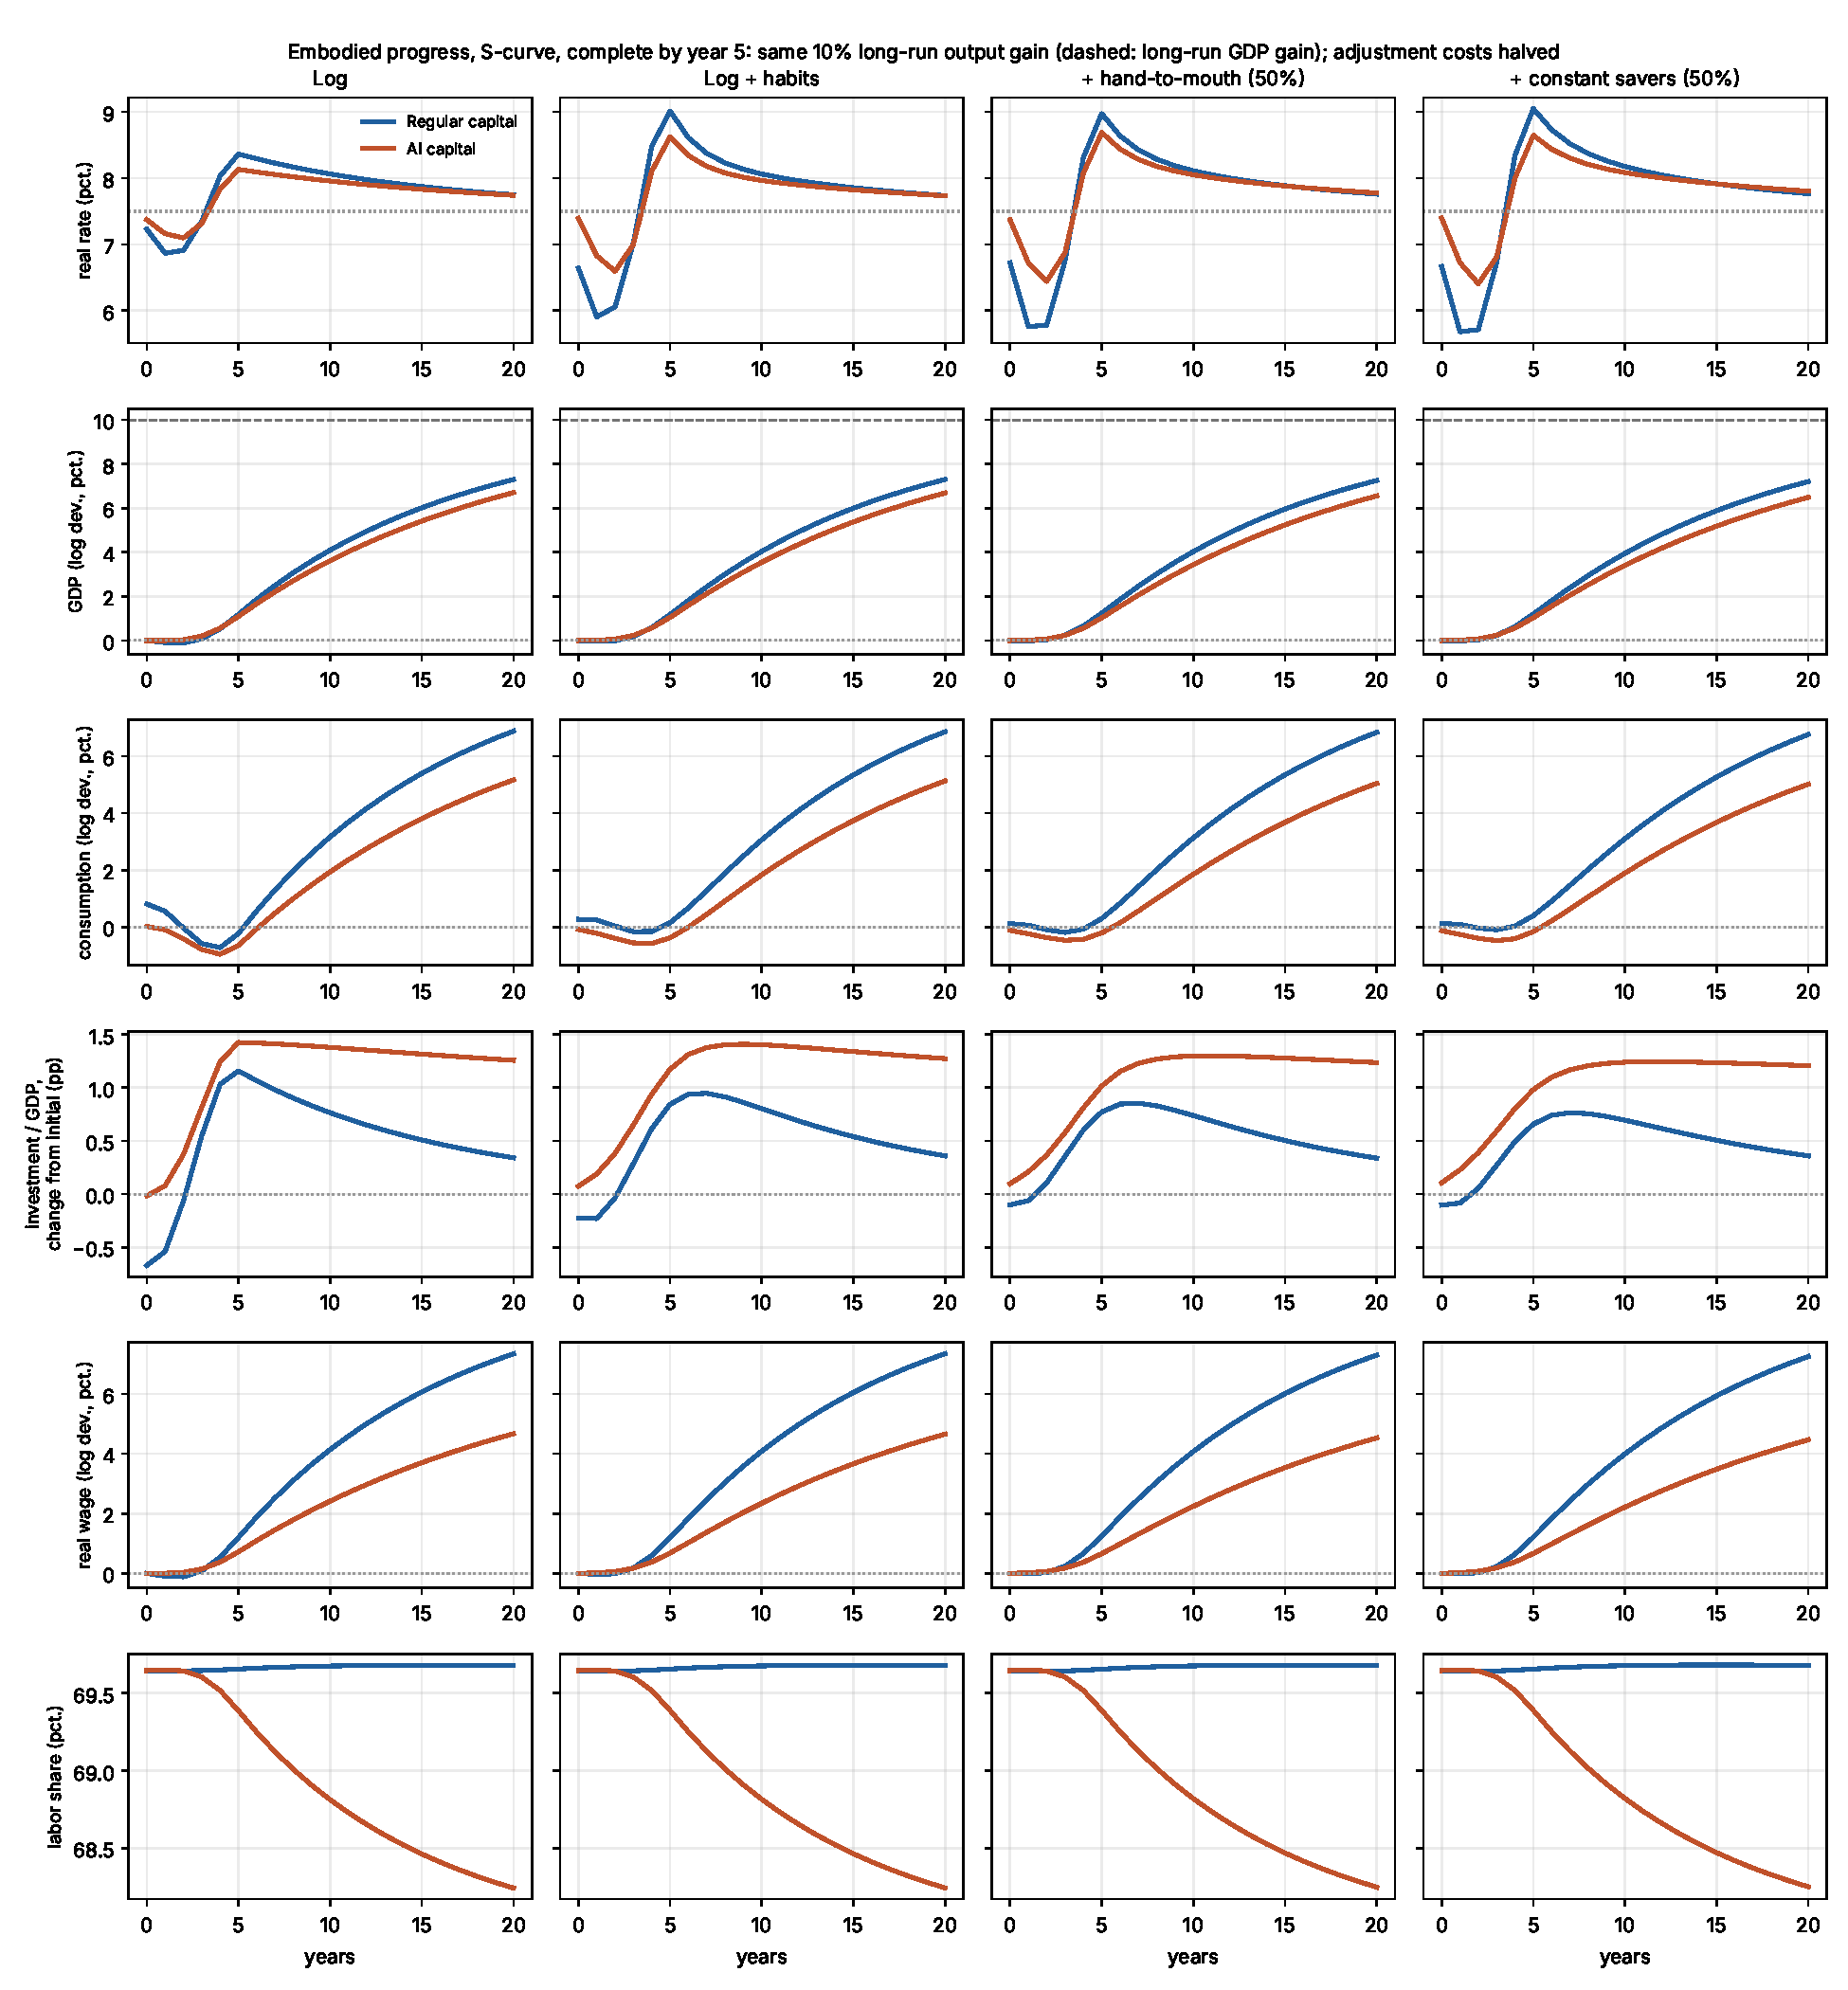
\includegraphics[width=0.93\textwidth]{figures/fig_emb_scurve.pdf}
\caption{Embodied progress, S-curve complete by year 5, same 10\% long-run output gain (dashed: long-run GDP gain). GDP, consumption and wages are log deviations from the pre-shock path. Investment/GDP includes adjustment costs.}\label{fig:scurve}
\end{figure}

\paragraph{Real side (log utility; similar across blocks).}
\begin{itemize}
\item \emph{GDP.} Regular capital is up 1.2 percent at year 5, 4.1 percent at year 10 and 7.3 percent at year 20. AI: 1.1, 3.6 and 6.7 percent.
\item \emph{Investment/GDP.} Firms wait for cheaper capital, so for regular capital the investment share \emph{falls} by 0.67 points at $t=0$ and then rises
by 1.16 points at year 5 (the end of the price decline), 0.76 at year 10 and 0.34 at year 20. For AI the share is flat initially, rises by 1.42 points at year 5, and stays 1.38 points higher at year 10 and 1.26 points higher at year 20.
\item \emph{Consumption.} It rises slightly early for regular capital (less is invested), dips below the pre-shock path around year 4 as investment picks up, and is 3.2 percent higher at year 10. For AI it is about 1.9 percent higher at year 10.
\item \emph{Wages and the labor share.} The wage is up 4.1 percent at year 10 for regular capital and 2.4 percent for AI. The AI labor share falls from 69.6 to 68.8 percent at year 10 and 68.2 percent at year 20.
Regular capital leaves it unchanged.
\end{itemize}

\paragraph{The real interest rate.} With these lower adjustment costs, firms respond more strongly to the announced price decline, and the wait-for-cheaper-capital response now appears for regular capital too.
\begin{itemize}
\item \emph{Log.} Regular capital: the rate falls to 6.9 percent in year 1 and then rises to 8.4 percent in year 5, when the technology is complete. AI: it falls to 7.1 percent in year 2 and rises to 8.1 percent in year 5.
Decade averages are +0.26 and +0.21 points relative to 7.5 percent.
\item \emph{Habits} sharpen both swings. Regular capital: trough 5.9 percent, peak 9.0 percent. AI: trough 6.6 percent, peak 8.6 percent. The decade averages (+0.15 and +0.22) are lower or similar, because the deeper trough offsets the higher peak.
\item \emph{Hand-to-mouth and constant savers} change little relative to habits alone. Regular capital: troughs 5.8 and 5.7 percent and peaks 9.0 and 9.05 percent. AI: troughs 6.4 and 6.4 percent and peaks 8.7 and 8.65 percent.
\end{itemize}

\begin{figure}[h]\centering
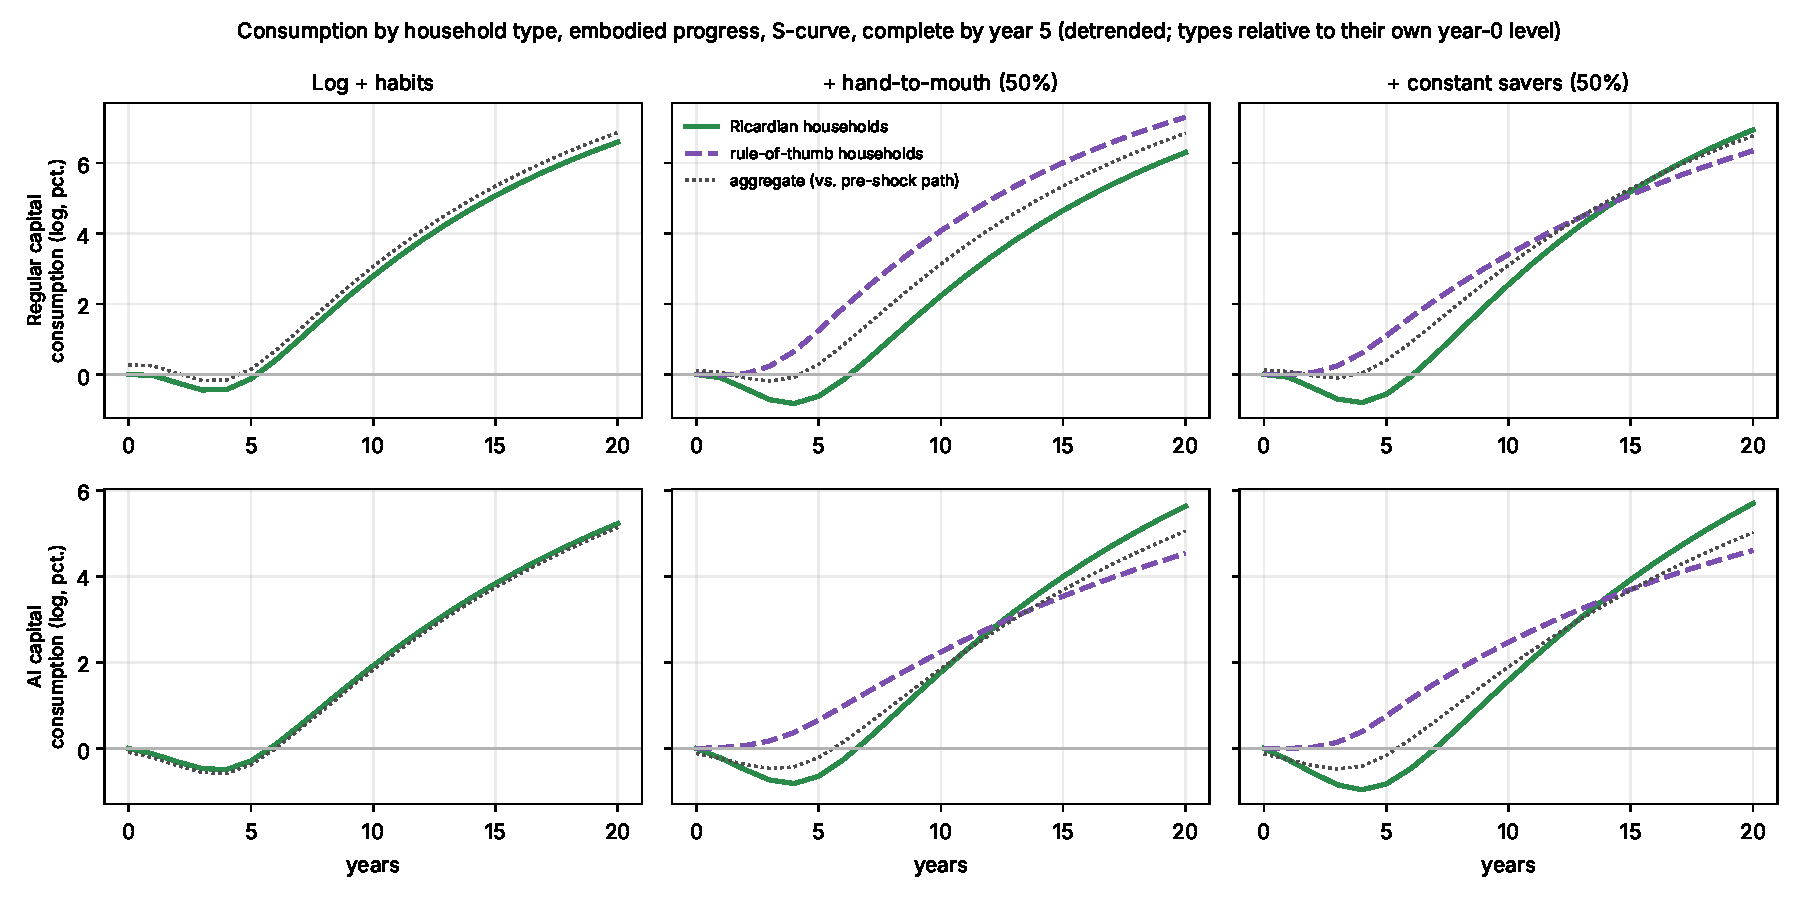
\includegraphics[width=0.95\textwidth]{figures/fig_emb_cons_scurve.pdf}
\caption{Consumption by household type, embodied progress, S-curve. Each type is shown relative to its own year-0 level; the dotted line is the aggregate relative to the pre-shock path.}\label{fig:cons}
\end{figure}

Figure~\ref{fig:cons} shows why the rule-of-thumb types matter so little. Hand-to-mouth consumption equals the wage bill. Under AI progress wages lag output (the labor share falls),
so hand-to-mouth consumption first exceeds, and later falls behind, the aggregate, and the Ricardian half does the opposite. Constant savers' income includes capital income, and their
consumption stays closer to the aggregate. In both cases the Ricardian half, which sets the rate, sees a path close to the aggregate, so the rate moves almost as under habits alone.

\section{A surprise jump}

\begin{figure}[p]\centering
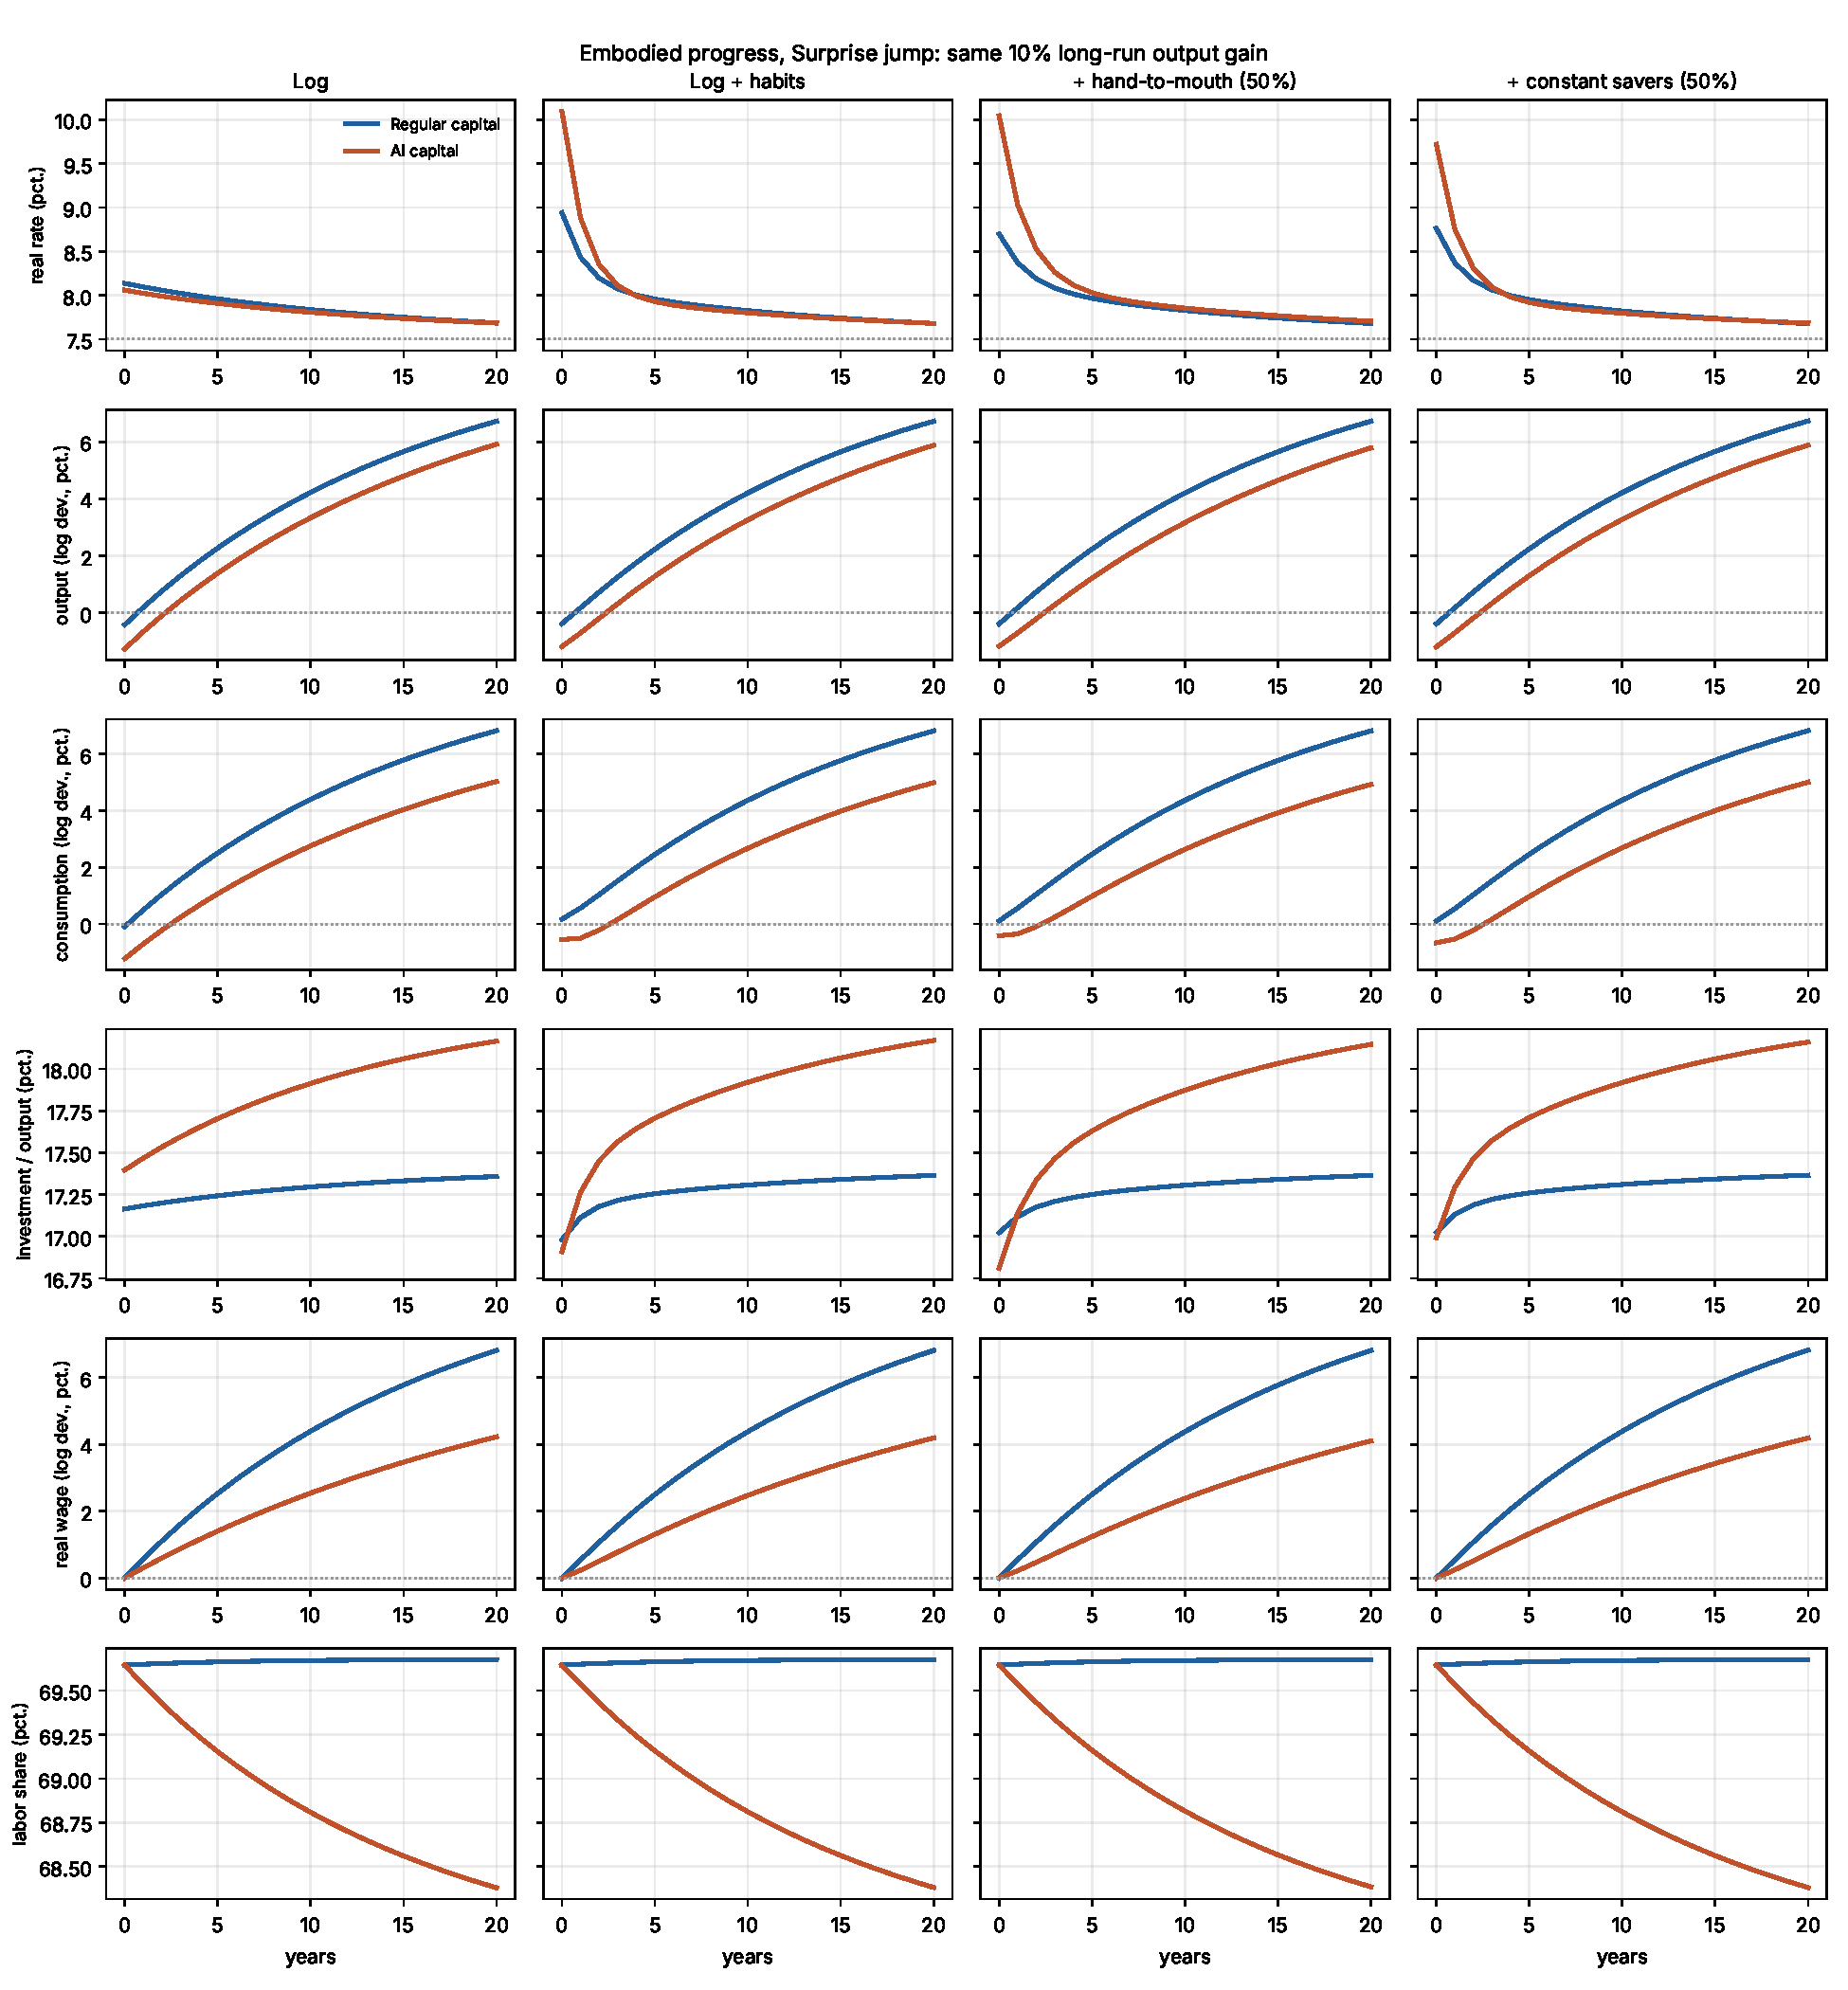
\includegraphics[width=0.93\textwidth]{figures/fig_emb_jump.pdf}
\caption{Embodied progress, surprise jump at $t=0$ (same layout as Figure~\ref{fig:scurve}).}\label{fig:jump}
\end{figure}

\begin{itemize}
\item \emph{GDP} does not move on impact (gross value added; $K$, $A$ and technology are predetermined or unchanged) and is up 3.3 percent (regular) and 2.9 percent (AI) at year 5, and 5.5 and 4.9 percent at year 10.
Consumption \emph{falls} on impact, by 1.6 and 1.7 percent under log utility and by 0.4 to 0.7 percent with habits, because the economy suddenly invests more.
\item \emph{Investment/GDP} rises on impact by 1.32 points (regular, log) and 1.43 points (AI). For regular capital the increase fades (0.87 at year 5, 0.58 at year 10, 0.26 at year 20), whereas for AI it persists (1.40 at year 5, 1.34 at year 10, 1.22 at year 20). With habits the rise is more gradual:
the peak is 0.98 points at year 3 for regular capital and 1.42 points at year 6 for AI.
\item \emph{The real rate} jumps on impact and decays. Log: 8.5 percent (regular) and 8.2 percent (AI); decade averages +0.69 and +0.54 points. Habits raise the impact rate to 10.3 and 9.9 percent (averages +1.04 and +0.87).
Hand-to-mouth gives 10.1 and 9.8 percent, and constant savers 10.0 and 9.6 percent, so the rule-of-thumb types lower the impact rate slightly relative to habits alone (by 0.1 to 0.3 points).
\end{itemize}
The half/half case lies between the pure cases (Table~\ref{tab:emb}).

\begin{table}[h]\centering\scriptsize
\caption{Embodied progress, by timing and household block. ``Decade avg.'' is the mean of $r_1,\dots,r_{10}$ minus 7.5\%. GDP is gross value added, and ``gap closed'' is GDP at year 10 as a percent of the 10\% long-run gain. The investment column is the peak change in investment/GDP (including adjustment costs) over the first 20 years, with the year in parentheses. Consumption is a log deviation from the pre-shock path.}\label{tab:emb}
\resizebox{\textwidth}{!}{\begin{tabular}{llcccccccc}\toprule
 & & decade avg. $r$ & $r_1$ & trough & peak (yr) & $\ln C$, yr 5 & $\ln C$, yr 10 & $\ln W$, yr 10 & $\ln Y$, yr 10\\
 & & (pp over 7.5\%) & (pct.) & (pct.) & (pct.) & (pct.) & (pct.) & (pct.) & (pct.)\\\midrule
S-curve & Regular: Log & +0.24 & 7.51 & 7.51 & 7.99 (9) & 0.4 & 2.2 & 2.2 & 1.9\\
 & Log + habits & +0.26 & 7.47 & 7.47 & 8.11 (9) & 0.4 & 2.2 & 2.2 & 1.9\\
 & + hand-to-mouth (50\%) & +0.25 & 7.47 & 7.47 & 8.10 (9) & 0.4 & 2.2 & 2.2 & 1.9\\
 & + constant savers (50\%) & +0.26 & 7.46 & 7.46 & 8.10 (9) & 0.4 & 2.1 & 2.2 & 1.9\\
\midrule
 & AI: Log & +0.09 & 7.50 & 7.50 & 7.89 (9) & -0.2 & 0.7 & 1.2 & 1.0\\
 & Log + habits & +0.12 & 7.70 & 7.41 & 8.09 (9) & -0.1 & 0.7 & 1.2 & 0.9\\
 & + hand-to-mouth (50\%) & +0.11 & 7.70 & 7.34 & 8.17 (9) & -0.1 & 0.8 & 1.1 & 0.9\\
 & + constant savers (50\%) & +0.12 & 7.69 & 7.43 & 8.06 (9) & -0.1 & 0.7 & 1.2 & 0.9\\
\midrule
Half/half & Regular: Log & +0.35 & 7.80 & 7.79 & 7.92 (9) & 1.4 & 3.3 & 3.3 & 3.1\\
 & Log + habits & +0.41 & 8.09 & 7.80 & 8.09 (0) & 1.4 & 3.2 & 3.3 & 3.0\\
 & + hand-to-mouth (50\%) & +0.38 & 7.96 & 7.80 & 7.98 (9) & 1.4 & 3.3 & 3.3 & 3.0\\
 & + constant savers (50\%) & +0.39 & 8.01 & 7.80 & 8.01 (0) & 1.4 & 3.2 & 3.3 & 3.0\\
\midrule
 & AI: Log & +0.22 & 7.70 & 7.65 & 7.87 (9) & 0.3 & 1.6 & 1.8 & 2.0\\
 & Log + habits & +0.35 & 8.48 & 7.63 & 8.48 (0) & 0.3 & 1.6 & 1.7 & 2.0\\
 & + hand-to-mouth (50\%) & +0.37 & 8.45 & 7.64 & 8.45 (0) & 0.4 & 1.6 & 1.7 & 1.9\\
 & + constant savers (50\%) & +0.32 & 8.32 & 7.64 & 8.32 (0) & 0.3 & 1.6 & 1.7 & 2.0\\
\midrule
Jump & Regular: Log & +0.48 & 8.14 & 7.86 & 8.14 (0) & 2.5 & 4.4 & 4.4 & 4.2\\
 & Log + habits & +0.61 & 8.94 & 7.85 & 8.94 (0) & 2.5 & 4.4 & 4.4 & 4.2\\
 & + hand-to-mouth (50\%) & +0.59 & 8.70 & 7.85 & 8.70 (0) & 2.5 & 4.4 & 4.4 & 4.2\\
 & + constant savers (50\%) & +0.58 & 8.76 & 7.84 & 8.76 (0) & 2.5 & 4.4 & 4.4 & 4.2\\
\midrule
 & AI: Log & +0.43 & 8.06 & 7.82 & 8.06 (0) & 1.1 & 2.8 & 2.5 & 3.3\\
 & Log + habits & +0.78 & 10.10 & 7.82 & 10.10 (0) & 1.0 & 2.7 & 2.5 & 3.3\\
 & + hand-to-mouth (50\%) & +0.87 & 10.04 & 7.88 & 10.04 (0) & 1.0 & 2.6 & 2.4 & 3.2\\
 & + constant savers (50\%) & +0.71 & 9.72 & 7.81 & 9.72 (0) & 1.0 & 2.7 & 2.5 & 3.3\\
\bottomrule\end{tabular}
}
\end{table}

\section{Summary and caveats}\label{sec:caveats}

\begin{enumerate}
\item \emph{Output builds slowly.} With gross-value-added GDP and half the earlier adjustment costs, GDP at year 10 is 45--55 percent of its long-run gain after a jump and 34--41 percent after a 5-year S-curve.
\item \emph{Investment rises persistently for AI and transitorily for regular capital.} The investment share of GDP rises by 1.2--1.4 points for AI, and the increase is still about 1.2 points after 20 years. For regular capital it rises by 0.8--1.3 points and fades.
Under an anticipated S-curve, regular-capital investment first falls.
\item \emph{Habits matter more for the real rate than rule-of-thumb consumers do.} They deepen the pre-arrival trough, raise the peak, and raise the impact response to a surprise by about 1.6--1.8 points.
\item \emph{Hand-to-mouth and constant savers give nearly the same results} (peaks and troughs within about 0.3 points of each other and of habits alone), because the Ricardian half still sees about the same consumption path as the aggregate.
\item \emph{AI versus regular capital:} AI has a smaller GDP and wage gain at year 10, a persistently falling labor share and a persistently higher investment share.
\end{enumerate}

\paragraph{Caveats.}
\begin{itemize}
\item The constant savers' behavior depends on the income definition. Two earlier versions were unsatisfactory. Net income with depreciation at current replacement cost mechanically raised capital income when $P$ fell, and with depreciation at base-year prices
the AI cases failed to solve. The present version uses a constant gross saving rate out of gross income and no depreciation term.
\item $h=0.7$ is a strong annual habit.
\item Adjustment costs are calibrated, not estimated. The earlier summary showed their level is the most important calibration choice for embodied progress.
\item Hours are fixed, there are no nominal rigidities, and the long-run real rate is pinned by the Ricardian Euler equation, so these results are about transitions.
\end{itemize}

\appendix
\section{Additional figures and verification}

\begin{figure}[h]\centering
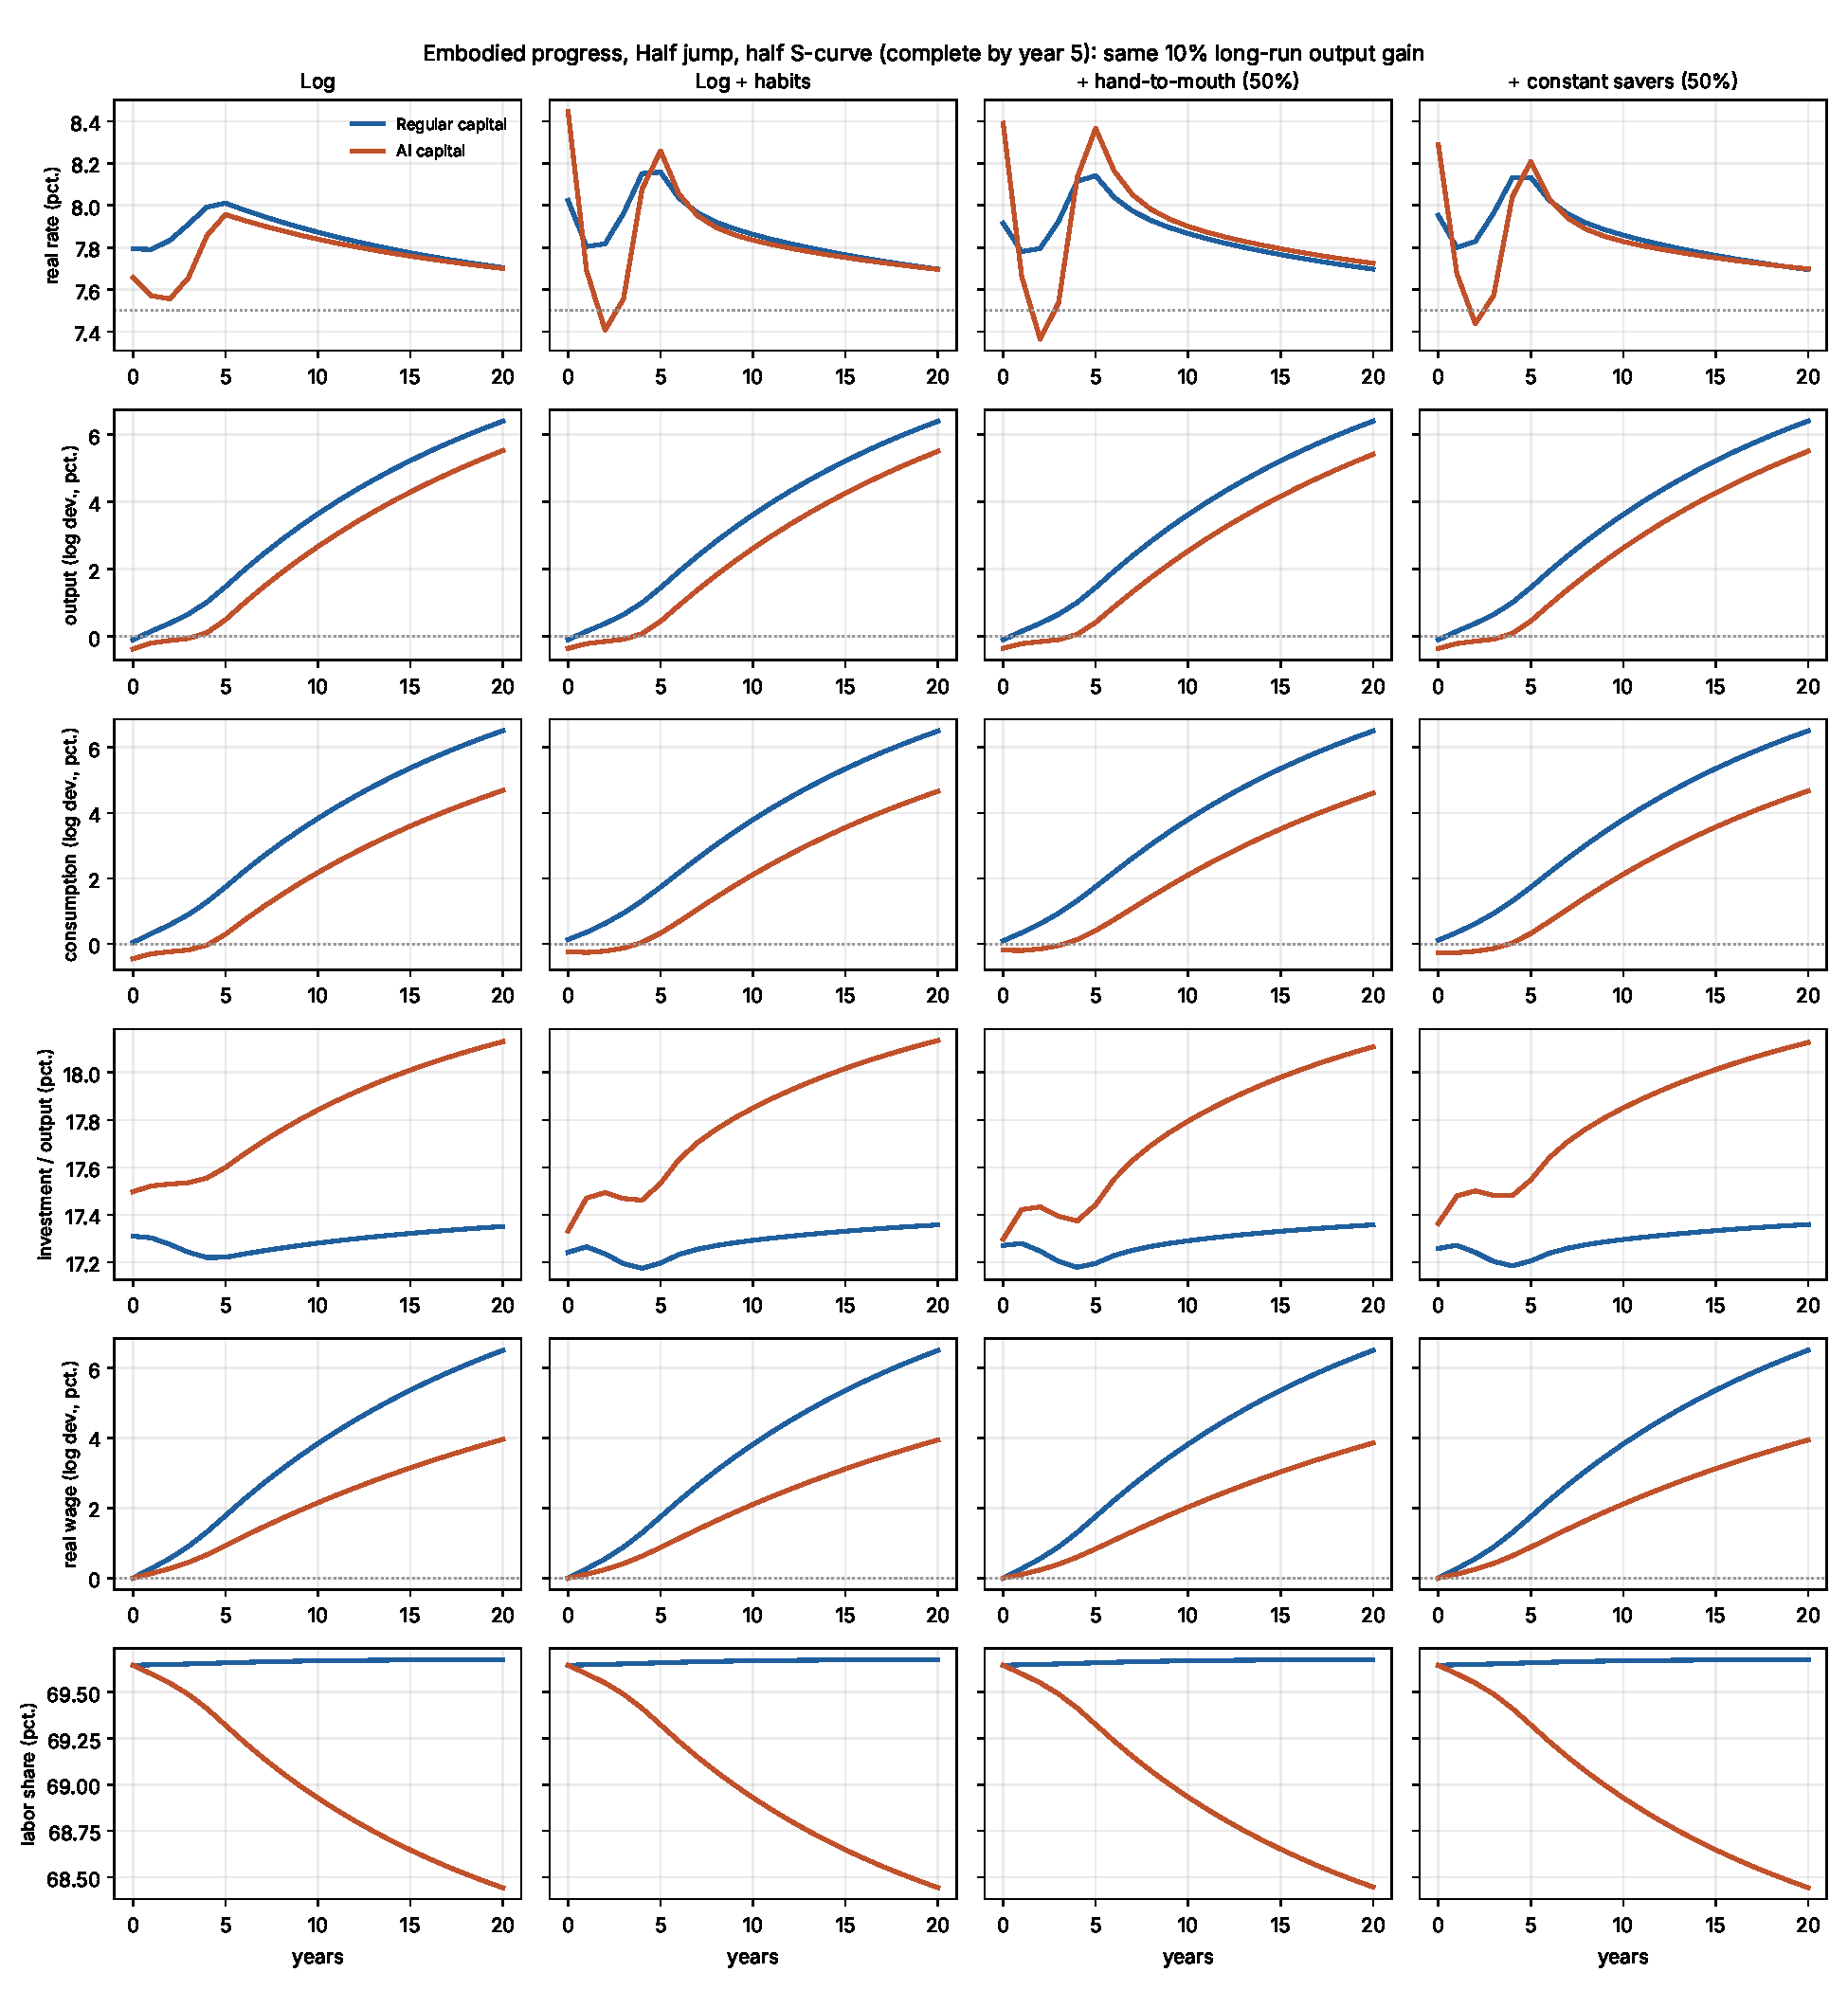
\includegraphics[width=0.9\textwidth]{figures/fig_emb_mixed.pdf}
\caption{Embodied progress, half jump and half 5-year S-curve.}
\end{figure}

\begin{figure}[h]\centering
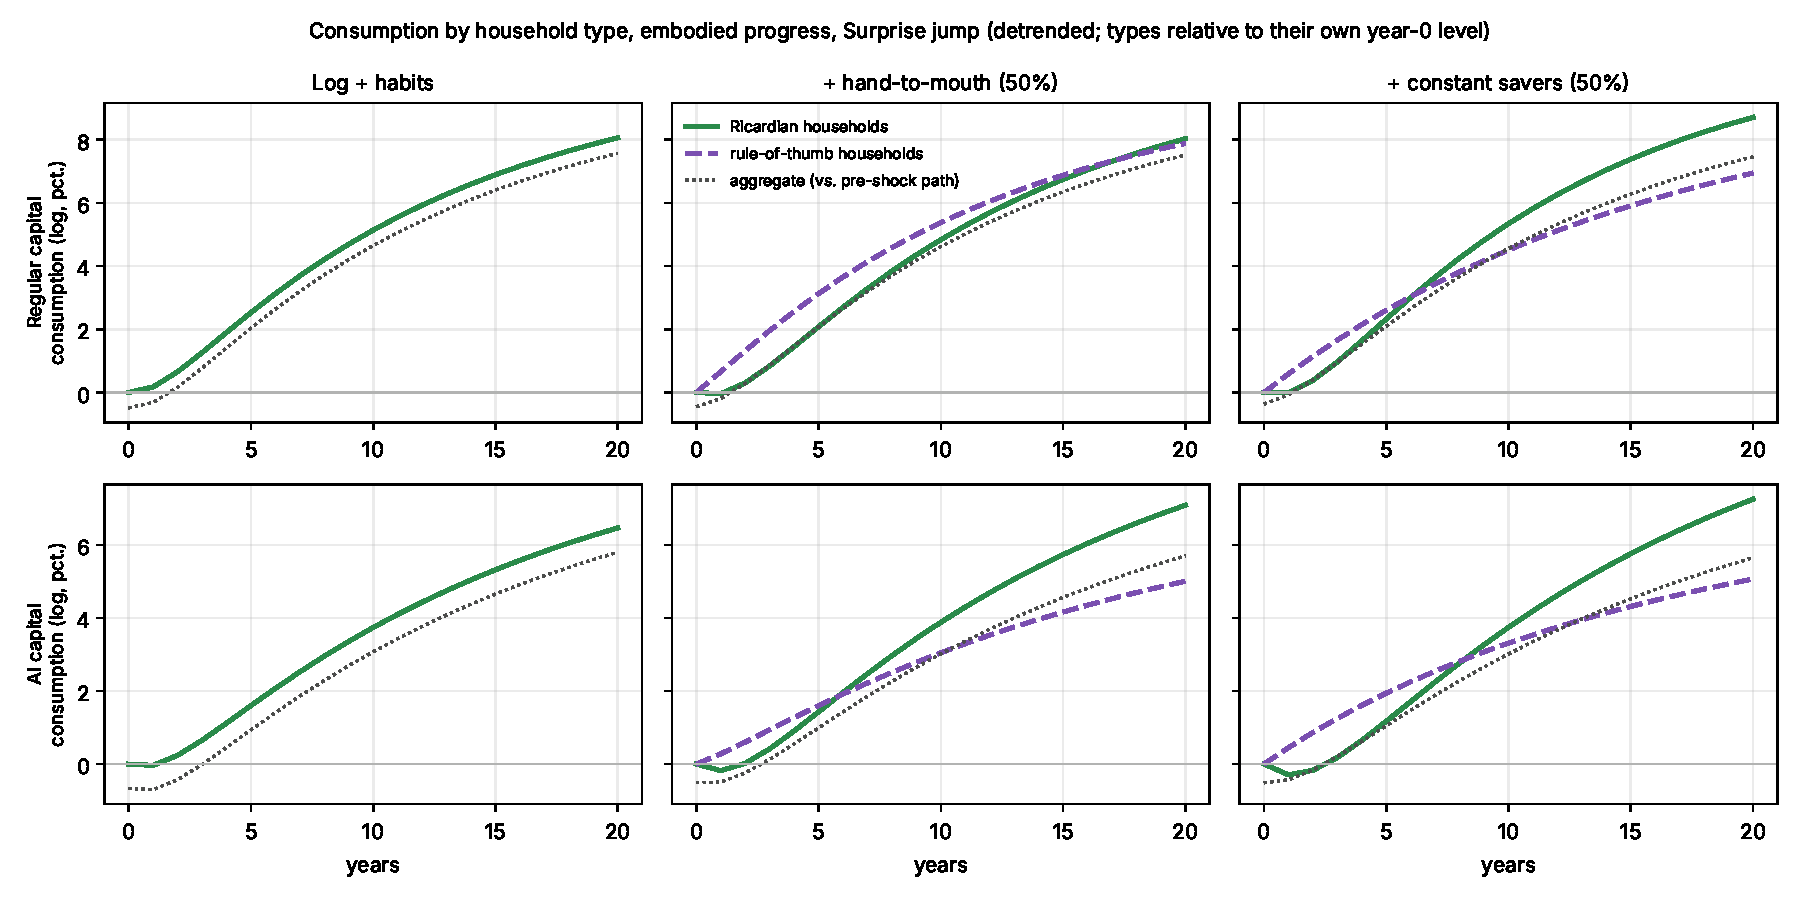
\includegraphics[width=0.95\textwidth]{figures/fig_emb_cons_jump.pdf}
\caption{Consumption by household type, embodied progress, surprise jump.}
\end{figure}

All results come from \texttt{embodied\_dynamics.py} (built on \texttt{ramsey\_variants.py} and \texttt{capital\_cases.py}). Each transition is a nonlinear
perfect-foresight solve over 250 years, warm-started from the previous household block. The saver block tracks the group's wealth recursively, and its wealth share stays between 0 and 1 throughout.

\begin{table}[h]\centering\scriptsize
\begin{tabular}{lc}\toprule Check & max abs. error\\\midrule
residual & 1.5e-11\\
long-run ln Y = 10\% & 2.8e-07\\
savers' wealth share within [0, 1] & 0.0e+00\\
BGP satisfies the Euler equations & 3.0e-14\\
\bottomrule\end{tabular}

\end{table}

\end{document}
